\documentclass[a4paper,12pt]{article}  %% important: a4paper first
% \usepackage[notcite,notref]{showkeys}
\pdfoutput=1
\usepackage{natbib} 
\usepackage{amsthm}
\usepackage{amssymb}
\usepackage{newpxtext,newpxmath} 
\usepackage{inconsolata} 
\usepackage{microtype}
\linespread{1.10}        % Palatino needs more leading (space between lines)
\usepackage{xcolor}
\usepackage{pict2e} 
% \usepackage{bimatrixgame}
\usepackage{tikz} 
\usetikzlibrary{shapes}
\usetikzlibrary{arrows.meta}
%\usepackage{smallsec}
\usepackage{graphicx}
%\usepackage[pdflatex]{hyperref}
\usepackage[hyphens]{url} 
\usepackage[colorlinks,linkcolor=blue,citecolor=blue]{hyperref}
%\usepackage{hyperref}
\urlstyle{sf}
\usepackage[format=hang,justification=justified,labelfont=bf,labelsep=quad]{caption} 
% \input macros-drawtree
\oddsidemargin=.46cm    % A4
\textwidth=15cm
\textheight=23.3cm
\topmargin=-1.3cm
\clubpenalty=10000
\widowpenalty=10000
\predisplaypenalty=1350
\sfcode`E=1000  % normal spacing if E followed by period, as in "EFCE."
\sfcode`P=1000  % normal spacing if P followed by period, as in "NP." 
\newdimen\einr
\einr1.7em
\newdimen\eeinr 
\eeinr 1.7\einr
\def\aabs#1{\par\hangafter=1\hangindent=\eeinr
    \noindent\hbox to\eeinr{\strut\hskip\einr#1\hfill}\ignorespaces}
\def\rmitem#1{\par\hangafter=1\hangindent=\einr
  \noindent\hbox to\einr{\ignorespaces#1\hfill}\ignorespaces} 
\newcommand\bullitem{\rmitem{\raise.17ex\hbox{\kern7pt\scriptsize$\bullet$}}} 
\def\subbull{\vskip-.8\parskip\aabs{\raise.2ex\hbox{\footnotesize$\circ$}}}
\let\sfield\mathcal
\newtheorem{theorem}{Theorem}
\newtheorem{corollary}[theorem]{Corollary}
\newtheorem{example}[theorem]{Example}
\newtheorem{lemma}[theorem]{Lemma}
\newtheorem{proposition}[theorem]{Proposition}
\theoremstyle{definition}
\newtheorem{remark}[theorem]{Remark}
\newtheorem{definition}[theorem]{Definition}
\def\reals{{\mathbb R}} 
\def\eps{\varepsilon}
\def\prob{\hbox{prob}}
\def\sign{\hbox{sign}}
\def\proof{\noindent{\em Proof.\enspace}}
\def\proofof#1{\noindent{\em Proof of #1.\enspace}}
\def\endproof{\hfill\strut\nobreak\hfill\tombstone\par\medbreak}
\def\tombstone{\hbox{\lower.4pt\vbox{\hrule\hbox{\vrule
  \kern7.6pt\vrule height7.6pt}\hrule}\kern.5pt}}
\def\eqalign#1{\,\vcenter{\openup.7ex\mathsurround=0pt
 \ialign{\strut\hfil$\displaystyle{##}$&$\displaystyle{{}##}$\hfil
 \crcr#1\crcr}}\,}
\def\zw#1\par{\vskip2ex{\textbf{#1}}\par\nobreak} 
\newsavebox{\figA} 
\parindent0pt
\parskip1.3ex

\newcommand{\T}{^{\top}}
\newcommand{\0}{{\mathbf0}}
\newcommand{\1}{{\mathbf1}}
\newcommand{\bezcontrol}[4]{\draw[dashed, ultra thick,green]
(#1) .. controls (#2) and (#3) .. (#4);
\draw[] (#1) circle [radius=0.01];
\draw[fill=pink] (#2) circle [radius=0.01];
\draw[] (#3) circle [radius=0.01];
\draw[] (#4) circle [radius=0.01];
\draw[brown] (#1) -- (#2);
\draw[brown] (#4) -- (#3);}
\newcommand{\bez}[4]{\draw[] (#1) .. controls (#2) and (#3) .. (#4);}

\title{%
Uniform Sampling from the Unit Simplex
}
\author{Bernhard von Stengel}
\date{February 3, 2025
%\\date{\today
\\[1ex]
}

\begin{document}
\maketitle

\begin{abstract}
We describe two simple methods to choose a point uniformly from
the unit simplex, and how round that point to a 
vector of fractions with a fixed limited denominator.
\end{abstract}

\section{Uniform sampling from the unit simplex}

% The $d$-dimensional \textit{unit simplex} $\Delta_d$ is
The \textit{unit simplex} $\Delta_n$ is
the convex hull of the $n$ unit vectors in
$\reals^{n}$, that is,
\[
\Delta_n=\{\,(x_1,\ldots,x_n)\mid
x_1+\cdots+x_n=1,~x_i\ge0~(1\le i\le n)\,\}\,.
\]
As a geometric object, $\Delta_n$ is a subset of $\reals^n$,
but has \textit{dimension} $n-1$ due to the equation.
For example, $\Delta_3$ is an equilateral triangle
(dimension~2), and $\Delta_4$ is
a regular tetrahedron (dimension~3).

We want to choose a point $x=(x_1,\ldots,x_n)$ in
$\Delta_n$ uniformly at random.
The naive method of choosing $n$ numbers uniformly from
the unit interval and dividing them by their sum
concentrates the points closer to the center of the simplex,
as in the following picture on the right for $n=3$:

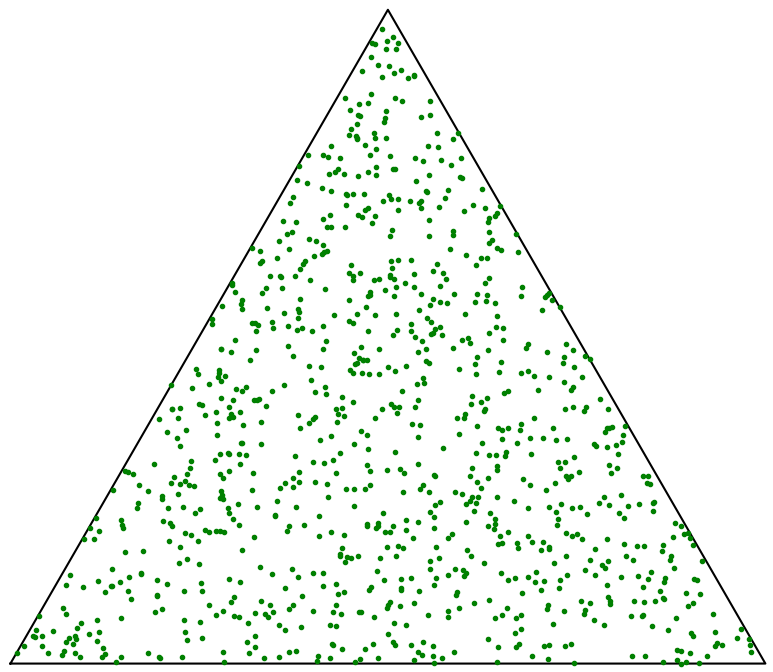
\includegraphics[width=.45\hsize]{1000.png}
\hfill
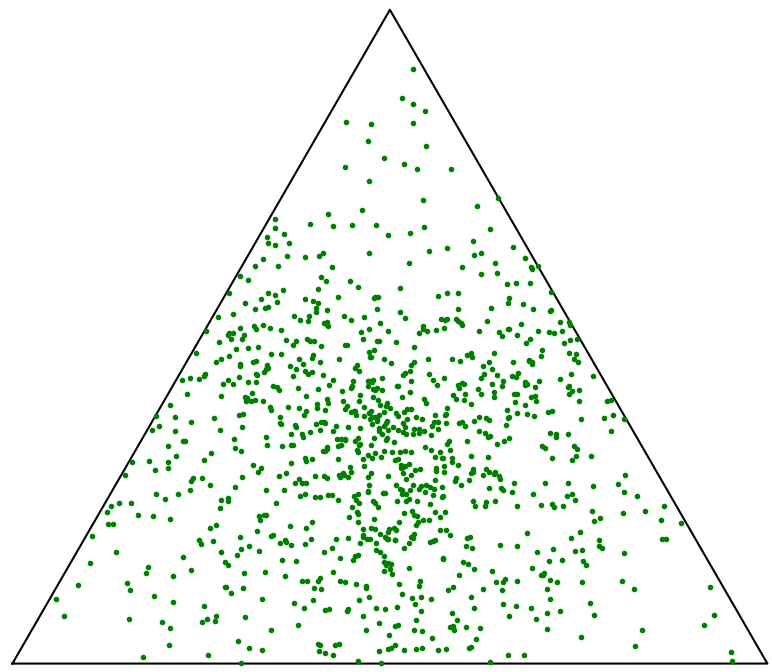
\includegraphics[width=.45\hsize]{naive1000.png}

The uniform distribution on the unit simplex is also known
as the ``flat Dirichlet distribution''.\footnote{%
See section XI.4 of
Devroye, L. (1986), Non-Uniform Random Variate Generation.
Springer, New York.
\url{https://luc.devroye.org/rnbookindex.html}
}
Instead of using a software package that generates points
from this distribution, we generate the coordinates 
$x_1,\ldots,x_n$ of a point $x$ in $\Delta_n$
recursively, starting with $x_n$.

If $x_n$ has value $t$ in $[0,1]$, this ``cuts off''
a small simplex of height $1-t$ from $\Delta_n$, as shown here
for $n=3$:
\[
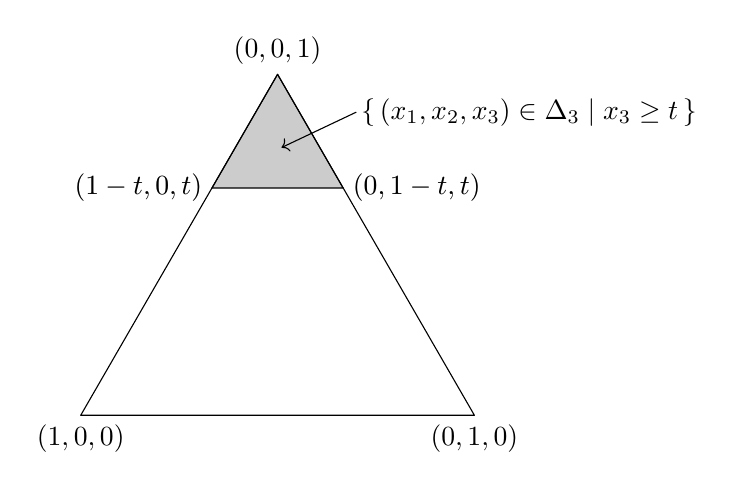
\begin{tikzpicture}[scale=5]
% \draw [help lines,color=green]  (-1,0) grid (1,1); 
% \draw [join=round] (-.5,0) node[below] {$e_0=(1,0,0)$}
   % -- (.5,0) node[below] {$e_1=(0,1,0)$} 
   % -- (0,.866) node[above] {$e_2=(0,0,1)$} -- cycle;
\draw [join=round] (-.5,0) node[below] {$(1,0,0)$}
   -- (.5,0) node[below] {$(0,1,0)$} 
   -- (0,.866) node[above] {$(0,0,1)$} -- cycle;
\draw [fill=black, fill opacity=0.2,join=round] 
   (-0.1666,0.5773) node[left] {$(1-t,0,t)$}
   -- (0.1666,0.5773) node[right] {$(0,1-t,t)$}
   -- (0,.866) -- cycle;
\draw [] (-0.1666,0.5773) node[left] {$(1-t,0,t)$};
\draw [] (0.1666,0.5773) node[right] {$(0,1-t,t)$};
% \draw [<-] (0.09,0.73) -- (0.2,0.77) node[right]
\draw [<-] (0.01,0.68) -- (0.2,0.77) node[right]
{\!\{\,$(x_1,x_2,x_3)\in\Delta_3\mid x_3\ge t\,\}$};
\end{tikzpicture}
\]
and $n=4$:
\[
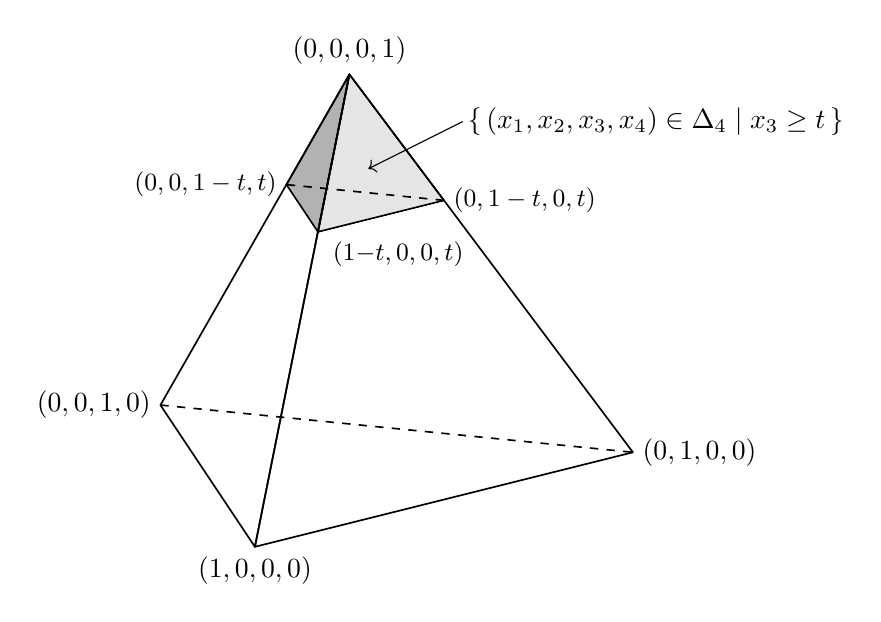
\begin{tikzpicture}[scale=1.2]
% \draw [help lines,color=green]  (-5,-3) grid (6,6);
\draw [semithick, join=round] (0,3) -- (-2,-.5) -- (-1,-2) -- cycle;
\draw [semithick, join=round] (0,3) -- (3,-1) -- (-1,-2) -- cycle; 
\draw [semithick, draw=black, fill=black, fill opacity=0.3,join=round] (0,3)
   -- (-.6666,1.8333)
   -- (-.333,1.333)
   -- cycle;
\draw [semithick, draw=black, fill=black, fill opacity=0.1,join=round] (0,3)
   -- (1,1.666) 
   -- (-.333,1.333)
   -- cycle;
\draw [dashed,semithick] (1,1.666) -- (-.6666,1.8333) ;
\draw [dashed,semithick] (-2,-.5) -- (3,-1);
% \draw (-1,-2) node[below] {$e_0$};
% \draw (3,-1)  node[right] {$e_1$};
% \draw (-2,-.5) node[left] {$e_2$};
% \draw (0,3)  node[above] {$e_3$};
\draw (-1,-2) node[below] {$(1,0,0,0)$};
\draw (3,-1)  node[right] {$(0,1,0,0)$};
\draw (-2,-.5) node[left] {$(0,0,1,0)$};
\draw (0,3)  node[above] {$(0,0,0,1)$};
\draw (-.6666,1.8333) node [left] {\small$(0,0,1-t,t)$};
\draw (1,1.666) node [right] {\small$(0,1-t,0,t)$};
\draw (-.333,1.333) node [below,xshift=29] {\small$(1{-}t,0,0,t)$};
% \draw [fill=blue] (-.6666,1.8333) circle [radius=0.07];
% \draw [fill=green] (-.333,1.333) circle [radius=0.07];
% \draw [fill=red] (0,0) circle [radius=0.07];
% \draw [fill=red] (1,1.666) circle [radius=0.07];
% \draw [fill=white] (-1,-2) circle [radius=0.07] node[below] {$e_0$};
% \draw [fill=white] (3,-1) circle [radius=0.07] node[right] {$e_1$};
% \draw [fill=white] (-2,-.5) circle [radius=0.07] node[left] {$e_2$};
% \draw [fill=white] (0,3) circle [radius=0.07] node[right,yshift=.2cm] {$e_3$};
% \draw (-1.5,2) node {$S$};
\draw [<-] (0.2,2.0) -- (1.2,2.5) node[right]
{\!\{\,$(x_1,x_2,x_3,x_4)\in\Delta_4\mid x_3\ge t\,\}$};
\end{tikzpicture}
\]
The volume of that cut-off simplex is the same as that of
$\Delta_n$ multiplied by $(1-t)^{n-1}$,
because it is the same $(n-1)$-dimensional geometric object
as $\Delta_n$ with each dimension reduced from $1$ to $1-t$.
The probability of $x$ being in that small simplex is
consequently given by that volume, that is, for our uniform
sampling
\begin{equation} \label{p}
\prob(x_n\ge t)=(1-t)^{n-1}\,.
\end{equation}
The cumulative distribution function $\prob(x_n\le t)$ is
therefore given by 
\begin{equation}
\label{cum}
\prob(x_n\le t)=1-(1-t)^{n-1},
\end{equation}
shown here for $n=3$ and $n=4$:

\begin{tikzpicture}[scale=5]
\draw []  (0,0) grid (1,1); 
\draw [->] (0,0) -- (1.1,0) node[right] {$t$};
\draw [->] (0,0) -- (0,1.1) node[above] {$\prob(x_3\ge t)$};
\draw[scale=1, samples=100, domain=0:1, variable=\x, blue] plot ({\x}, {1-(1-\x)^2});
% \bez{0,0}{0.3333,0.6666}{0.6666,1.0}{1,1};
\draw[dashed] (0,0.8) -- (0.5528,0.8) -- (0.5528,0);
\draw[] (-.02,0.8) node[left]{$b$} -- (0,0.8);
\draw[] (0.5528,0) -- (0.5528,-.02) node[below]{$x_3$};
\end{tikzpicture}
\hfill
\begin{tikzpicture}[scale=5]
\draw []  (0,0) grid (1,1); 
\draw [->] (0,0) -- (1.1,0) node[right] {$t$};
\draw [->] (0,0) -- (0,1.1) node[above] {$\prob(x_4\ge t)$};
\draw[] (-.02,0.8) node[left]{$b$} -- (0,0.8);
\draw[dashed] (0,0.8) -- (0.4152,0.8) -- (0.4152,0);
\draw[] (0.4152,0) -- (0.4152,-.02) node[below]{$x_4$};
\draw[scale=1, samples=100, domain=0:1, variable=\x, blue] plot ({\x}, {1-(1-\x)^3});
%\bezcontrol{0,0}{0.3333,1}{0.6666,1.0}{1,1};
\end{tikzpicture}

These pictures describe how to find the proper random value
of $x_n$ from the cumulative distribution function
(\ref{cum}):
Choose the vertical value $b$ of the function $1-(1-t)^{n-1}$
uniformly at random from $[0,1]$ and then determine $x_n=t$
according to $b=1-(1-t)^{n-1}$, that is, 
\begin{equation}
\label{1-b}
(1-b)^{1/{(n-1)}}=1-x_n
\end{equation}
where we can just as well choose $1-b$ rather than $b$
uniformly from $[0,1]$, giving 
\begin{equation}
\label{b}
1-x_n=b^{1/(n-1)}.
\end{equation}
With $x_n$ randomly chosen in that way,
the remaining
coordinates $x_1,\ldots,x_{n-1}$ belong to a
scaled version of $\Delta_{n-1}$ (the ``bottom'' of the
``cut-off tip'' of $\Delta_n$) where the side of
each edge is shrunk from length $1$ to $1-x_n$.
We then determine $x_{n-1}$ by sampling from the simplex 
$\Delta_{n-1}$ of the next-smaller dimension,
except that all coordinates are multiplied by
% $1-x_n$\,, shown as \verb.f. in this Python method:
$1-x_n$\,, shown as \verb.f. in the Python method below.
% The above Python method computes $(x_1,\ldots,x_n)$, per
The method computes $(x_1,\ldots,x_n)$, per
standard convention, as a 
list with entries \verb.x[0]., \ldots, \verb.x[n-1]..
It first computes \verb.x[n-1]., and then recursively
\verb.x[n-2]., \ldots, \verb.x[0]. in successively smaller
dimensions, except that these components have a smaller sum
given by the variable \verb.factor., which at the beginning
of each iteration of the \verb.while. loop equals
$x_0+\cdots+x_{i}$\,, starting with $i=n-1$.
The method iterates down to $i=1$, and finally sets \verb.x[0].
as the remaining value of \verb.factor..

\vbox{%
{\small
\begin{verbatim}
import random
def randInSimplex(n):
    x = [0.0]*n
    factor = 1.0
    i = n-1
    while i>0:
        b = random.uniform(0, 1)
        f = b**(1/i)
        x[i] = factor * (1-f)
        factor *= f
        i -= 1
    x[0] = factor
    return x
\end{verbatim}}}

\section{Logarithms of i.i.d.\ uniform variables}

Surprisingly, we can also generate a uniform distribution
on the unit simplex $\Delta_n$ by the following fully
symmetric method:
Choose independently $n$ variables
$y_1,\ldots,y_n$ uniformly at random from the interval
$[0,1]$ (assuming that $0$ and $1$ will not be chosen), take
their \textit{logarithms}, and normalize them so that they
sum to~$1$ (the base of the logarithm doesn't matter).
That is, $x=(x_1,\ldots,x_n)$ is computed from 
$(y_1,\ldots,y_n)$ via
\begin{equation}
\label{xy}
x_i= \frac{\log y_i}{\sum_{k=1}^n \log y_k}
\qquad (1\le i\le n).
\end{equation}
The claim is that then $x$ is uniformly chosen from
$\Delta_n$.
The corresponding Python method is this:

{\small
\begin{verbatim}
import math 
import random
def randInSimplex(n):
    y = [0.0]*n
    sum = 0.0
    for i in range(n):
        y[i] = math.log(random.uniform(0, 1))
        sum += y[i]
    return [z/sum for z in y] 
\end{verbatim}}

Apparent from similar pictures to those above, this clearly works.
But why?
We prove this with standard first-year mathematics.\footnote{%
This was asked at
\url{https://math.stackexchange.com/questions/4235192/prove-this-method-generates-uniform-points-on-the-simplex}, with my answer now added there.
See also (without proof)
\url{http://blog.geomblog.org/2005/10/sampling-from-simplex.html}} 

The vector $y=(y_1,\ldots,y_n)$ is chosen uniformly from the
$n$-dimensional unit cube $[0,1]^n$. 
With $x$ as defined in (\ref{xy}), we want to show
(\ref{p}).

By (\ref{xy}), we have the following equivalences
(note that all logarithms are negative):
\renewcommand{\arraystretch}{1.5}
\[
\begin{array}{rcl}
x_n&\ge& t\\
\log y_n/\sum_{k=1}^n \log y_k&\ge& t\\
\log y_n&\le& t\sum_{k=1}^n \log y_k\\
\log y_n(1-t)&\le& t\sum_{k=1}^{n-1} \log y_k\\
\log y_n&\le&\sum_{k=1}^{n-1} \frac t{1-t} \log y_k\\
y_n&\le& \prod_{k=1}^{n-1} y_k^{t/(1-t)}\\
\end{array}
\]
where the equation 
\[
y_n=\prod_{k=1}^{n-1} y_k^{t/(1-t)}
\]
defines $y_n$ as a function of $y_1,\ldots,y_{n-1}$,
that is, a surface in the cube $[0,1]^n$  that is ``above'' the facet
of the cube given by the points $(y_1,\ldots,y_{n-1},0)$.
The cube itself has volume~$1$, hence $\prob(x_n\ge t)$ is
the volume below that surface, given by the following
multiple integral, where we use that $t/(1-t)=
1/(1-t)-1$ (it helps to visualize first the case $n=2$):
\[
\begin{array}{rcl}
\prob(x_n\ge t)&=&\int_0^1\int_0^1\cdots\int_0^1\prod_{k=1}^{n-1} y_k^{t/(1-t)}
dy_{n-1}\cdots dy_2\,dy_1
\\[1ex]
&=&\left(\int_0^1 z^{t/(1-t)}dz\right)^{n-1}\\[1ex]
&=&\left(\left[\frac 1{1/(1-t)}z^{1/(1-t)}\right]^{z=1}_{z=0}\right)^{n-1}\\
&=&(1-t)^{n-1}\\
\end{array}
\]
which proves (\ref{p}).
Because (\ref{xy}) is symmetric in all components, 
we have more generally for all $i=1,\ldots,n$ that
\[
\prob(x_i\ge t)=(1-t)^{n-1}\,.
\]

\section{Rounding points in the simplex to small fractions}

The points $(x_1,\ldots,x_n)$ in $\Delta_n$ are
floating-point numbers.
We use them as mixed strategies that define starting points in
computations for finding Nash equilibria in two-player
games, where we need fractions whose denominator does
not exceed a certain size~$h$, say.
Hence, we need to round each $x_i$ to a fraction $p_i/h$
with numerator $p_i$ such that $p_1+\cdots+p_n=h$.
This problem has been studied as the \textit{apportionment}
of an integer number $p_i$ of seats to each party with vote
fraction~$x_i$ in a house of parliament with $h$ seats
in total.\footnote{Balinski,
M. L. and H. P. Young (1994), Apportionment. In: S. M. Pollock et al, eds,
\textit{Handbooks in Operations Research and Management
Science} Vol. 6, Chapter~15, 529--560.}
There are various methods for this, which can vary
significantly if $h$ is small, such as $h=10$ (see below).
For our application, typically $h=10000$, and the choice of
method is irrelevant.

We choose the following: Let $q_i= x_i\,h$ be
the ideal quota for each party $i=1,\ldots,n$,
and consider its integer part $\lfloor q_i\rfloor$
as the minimum number of seats for that party.
The resulting total remainder
$r=\sum_{i=1}^n (q_i-\lfloor q_i\rfloor)=
h-\sum_{i=1}^n \lfloor q_i\rfloor$ fulfills $0\le r<n$.
We set $p_i=\lfloor q_i\rfloor+1$ for the $r$ parties with
the largest remainders
$q_i-\lfloor q_i\rfloor$, 
and $p_i=\lfloor q_i\rfloor$ for rest.
Then $p_1+\cdots+p_n=h$ as required.

For example, let $n=3$ and $(x_1,x_2,x_3)=(0.756,0.164,0.08)$
and $h=10$. Then $(q_1,q_2,q_3)=(7.56,1.64,0.8)$ and $r=2$.
The described method of largest remainders gives
$(p_1,p_2,p_3)=(7,2,1)$.
The method is known to favor smaller parties.
However, it also has a non-monotonicity called the ``Alabama
paradox'' where increasing $h$ can lead to a lower value of
some $p_i$ (which is irrelevant for our application where
$h$ is fixed).
The different ``d'Hondt'' method favors large parties.
For the above example, it gives $(p_1,p_2,p_3)=(9,1,0)$ where both
extra seats go to the largest party, in excess of its
``natural'' quota that only allows $p_1=7$ or $p_1=8$.

% \bibliographystyle{book}
% \bibliography{bib-evol} 

\end{document}

